\documentclass[pdflatex,sn-basic,referee]{sn-jnl}

\usepackage{graphicx}
\usepackage{amsmath,amssymb,amsfonts}
\usepackage{textcomp}
\usepackage{xcolor}
\usepackage{booktabs}
\usepackage{microtype}
\usepackage{tabularx}
\usepackage{array}
\hypersetup{hidelinks}

\makeatletter
\renewcommand{\email}[1]{%
  \global\advance\emailcnt by 1\relax
  \if@corauemail
    \g@addto@macro\corrauthemail{%
      \setcounter{footnote}{0}%
      \textcolor{blue}{#1}\ %
    }%
  \else
    \g@addto@macro\authemail{%
      \setcounter{footnote}{0}%
      \textcolor{blue}{#1};\ %
    }%
  \fi
}
\makeatother

\newcommand{\tabtworow}[2]{\begin{tabular}[t]{@{}>{\raggedright\arraybackslash}p{1.75cm}@{}}#1\\[-2pt]{\small #2}\end{tabular}}

\begin{document}

\title[Context as a Budget]{Context as a Budget: A Taxonomy, an Accounting Framework, and a Measurement Audit for Composing Token-Efficiency Interventions in {LLM} Agents}

\author*[1]{\fnm{Soumitra} \sur{Mehrotra}}\email{soumitra.mehrotra9@gmail.com}

\author[1]{\fnm{Shubhender} \sur{Singh}}\nomail

\author[1]{\fnm{Saurabh} \sur{Aggarwal}}\nomail

\affil*[1]{\orgaddress{\city{San Francisco}, \country{USA}}}

\abstract{Large language model (LLM) agents consume a shared context budget that grows across turns through tool schemas, execution output, conversation history, and model reasoning. Many methods reduce this budget, but their published evaluations use different tasks and metrics and never test whether savings from methods in different parts of the pipeline compose. This paper asks a prior question: what does it cost to measure composition at all? We contribute (i) a taxonomy of fourteen in-scope interventions across five intervention points with eight comparison axes; (ii) a budget-recurrence accounting framework that expresses each category's savings in a common unit and yields testable predictions; and (iii) a measurement audit built from a preregistered $2{\times}2$ factorial pilot on a self-hosted coding agent. The audit is the central result. Cumulative prompt tokens have a per-cell standard deviation about equal to their mean ($\approx$62{,}700 versus $\approx$58{,}900), driven by task success or failure. Across eighteen token-outcome contrasts, only two are distinguishable from zero, and both are treatment-fidelity checks that confirm each intervention did the mechanical thing it is defined to do: output filtering cuts tool output ($-803$ tokens, $|t|=2.26$) and compaction cuts cumulative prompt tokens ($-23{,}495$, $|t|=2.08$). Neither survives multiplicity correction, and no compositional or downstream effect is detectable. When a design can barely detect its own manipulation, it cannot detect a second-order interaction between two manipulations. We quantify the requirement: resolving the observed output-filtering prompt-token effect would need roughly 4{,}900 runs per cell, against the twelve used here. We also document two reusable evaluation diagnostics: 72\% of a nominal 144-run experiment carried no information because runs were process-degenerate in a treatment-loaded pattern, and expanding from two to six random seeds bought only about one extra distinct trajectory per cell at temperature 0.2. The contribution is the framework together with the measured cost of running this class of evaluation correctly, with the pilot as the worked example.}

\keywords{agent evaluation, composition study, context window, measurement, statistical power, systematization of knowledge, token efficiency}

\maketitle

\section{Introduction}

Schema injection across 308 Model Context Protocol (MCP) servers requires 248{,}100 prompt tokens per request~\citep{mcpzero2025}. Schema bloat inflates prompt token counts by more than 50\% on small tool sets~\citep{ragmcp2025}. Qwen2.5-14B-Instruct generates a mean of 313 tokens to solve a single GSM8K arithmetic problem~\citep{tokenskip2025}. Together, these examples show that schemas, tool interfaces, and explicit reasoning can each consume a substantial context budget.

The problem has attracted significant attention. RAG-MCP~\citep{ragmcp2025} measures selection accuracy and prompt tokens. TokenSkip~\citep{tokenskip2025} measures arithmetic benchmark accuracy at different compression ratios. Ponytail~\citep{ponytail2025} measures lines of code, session tokens, and task completion time simultaneously. These are not comparable units. We identified no evaluation in the combined defined corpus that activates methods from different intervention-point categories within the same agent trajectory (Section~\ref{sec:claims}).

The natural next question is whether savings from methods in different categories compound when stacked. Answering it requires a composition experiment: run each method alone and together and measure the interaction. Before running such a study at scale, a prior question must be settled, and it is the question this paper is built around: \emph{what does it cost to measure composition at all?} The outcome that composition acts on is session-level token consumption, and in agent trajectories that quantity is dominated by whether the task succeeds or fails. Failed runs accumulate several times more tokens than successful ones, so the between-run variance of cumulative tokens is enormous relative to any plausible interaction effect. If a modestly sized factorial cannot resolve the effect it is designed to detect, then the many single-method ``$X$\% savings'' numbers in the literature, reported without power analysis, rest on shakier ground than they appear to.

We take this question seriously by running a preregistered $2{\times}2$ factorial pilot on a self-hosted coding agent and then auditing what it could and could not detect. The audit is the paper's central exhibit. Cumulative prompt tokens have a per-cell standard deviation about equal to their mean. Of eighteen token-outcome contrasts, only two clear zero, and both are manipulation checks rather than findings: they confirm each intervention mechanically did what it is defined to do. No compositional or downstream effect is detectable, and resolving even the effect we do observe would require thousands of runs per cell. We treat this not as a null result to be explained away but as a measured property of the evaluation itself: this is what it costs to do the measurement honestly.

The contributions of this paper are:
\begin{enumerate}
\item A taxonomy of fourteen in-scope interventions across five categories, plus two excluded boundary cases, with eight comparison axes (Section~\ref{sec:taxonomy}, Table~\ref{tab:taxonomy}).
\item A budget-recurrence accounting framework (Section~\ref{sec:background}) that expresses each category's savings in a common unit and, unlike a descriptive decomposition, yields a priori predictions; we test one such prediction and report the test as inconclusive at this sample size.
\item An evidence audit of the corpus: no strict two-method cross-category composition with individual baselines was found (C1, restated with its limitations), published evaluations are not directly commensurable (C2), and savings exhibit asymmetric recurrence depending on intervention point (C3) (Section~\ref{sec:claims}).
\item A measurement audit (Section~\ref{sec:composition}) that quantifies what evaluating composition in this setting costs: cumulative-token variance approximately equal to the mean, no detectable compositional effect, treatment fidelity that itself barely clears detection, and the sample size (roughly 4{,}900 runs per cell) required to resolve the observed effect.
\item Two reusable evaluation diagnostics (Section~\ref{sec:composition}): a process-based degeneracy filter that flagged 72\% of a nominal 144-run experiment as uninformative in a treatment-loaded pattern, and evidence that seed expansion buys little trajectory diversity at low temperature.
\end{enumerate}

Section~\ref{sec:background} establishes notation and scope. Section~\ref{sec:anatomy} decomposes the prompt budget empirically. Section~\ref{sec:taxonomy} presents the taxonomy. Section~\ref{sec:claims} states the three structural claims. Section~\ref{sec:composition} reports the composition study. Section~\ref{sec:discussion} discusses implications and limitations. Section~\ref{sec:related} compares related work. Section~\ref{sec:conclusion} concludes.

\section{Background and Scope}
\label{sec:background}

\subsection{Notation}

We write $B_t$ for prompt tokens serialized at turn $t$; $\mathrm{GT}_t$ for tokens generated at turn $t$; $\mathrm{PO}=\max_t B_t$ for peak occupancy; $\tau$ for the compaction trigger threshold; and $\hat{\Delta}$ for the $2\times2$ factorial interaction estimand (Section~\ref{sec:composition}). We use \emph{prompt-token cost} for serialized context consumption and \emph{generated-token cost} for model output; \emph{token consumption} refers to both. Inference-side metrics (KV-cache utilization, memory bandwidth, speculative decoding efficiency) are outside scope.

\subsection{Scope Exclusions}

MemGPT-style memory management~\citep{memgpt2023} re-architectures the budget (extends effective context rather than reducing per-turn cost) and is therefore a distinct problem class. Latent chain-of-thought methods such as Coconut~\citep{coconut2024} change the accounting substrate---savings accrue in forward passes, not context tokens---and cannot be expressed in the same unit as any other method in the taxonomy. We exclude both because they alter the accounting substrate rather than reducing serialized context tokens.

\subsection{Budget Model and Recurrence}

Let $S$ denote the scaffolding token count (system prompt, task instruction, tool schema---constant across turns). Let $H_i = A_i + O_i + U_i$ denote the tokens retained from turn $i$, where $A_i$ are assistant-generated tokens, $O_i$ are tool-output tokens, and $U_i$ are other retained conversational tokens. Then the prompt budget at turn $t$ without compaction is
\begin{equation}
  B_t = S + \sum_{i=1}^{t-1} H_i
  \label{eq:budget}
\end{equation}
After a compaction event at turn $q$, content accumulated through turn $q$ is replaced by a summary $C_q$:
\begin{equation}
  B_t = S + C_q + \sum_{i=q+1}^{t-1} H_i, \qquad t > q
  \label{eq:budget_post}
\end{equation}
Compaction reduces occupancy when
\begin{equation}
  C_q < \sum_{i=1}^{q} H_i
  \label{eq:compaction_constraint}
\end{equation}
and is not applied otherwise. This decomposition connects the taxonomy directly to the model: Category~1 acts on $S$; Category~2 acts on $O_i$; Category~3 replaces accumulated $H_i$ with $C_q$; Category~4 acts primarily on $A_i$; Category~5 may alter $A_i$, downstream $O_i$, and total trajectory length $T$.

A reduction $\Delta S$ to scaffolding recurs at every turn:
\begin{equation}
  \Delta_{\mathrm{PT}}^{(S)} = \Delta S \cdot T
  \label{eq:scaffold_savings}
\end{equation}
where $T$ is the total number of turns in the session. A reduction $\Delta O_k$ to tool-output tokens at turn $k$ (Category~2) produces the same recurrence form as a retained generation reduction:
\begin{equation}
  \Delta_{\mathrm{PT}}^{(O,k)} = \Delta O_k \cdot (T - k)
  \label{eq:toolout_savings}
\end{equation}
A reduction $\Delta A_k$ to assistant-generated tokens at turn $k$, as in Category~4 and in some Category~5 interventions, produces:
\begin{equation}
  \Delta_{\mathrm{PT}}^{(A,k)} = \Delta A_k \cdot (T - k)
  \label{eq:gen_savings}
\end{equation}
Whenever $\Delta O_k = \Delta S$ and $k > 0$, $\Delta_{\mathrm{PT}}^{(O,k)} < \Delta_{\mathrm{PT}}^{(S)}$, with the gap widening as $k \to T$. This is not a novel mathematical result; it is a formal statement of a relationship implicit in every individual method paper but never stated explicitly across categories. It is the basis for claim C3 (Section~\ref{sec:claims}).

For a $T$-turn session, the ratio of accumulated PT savings from an equal-sized scaffolding reduction versus a tool-output or generation reduction at turn $k$ is
\begin{equation}
  \frac{\Delta_{\mathrm{PT}}^{(S)}}{\Delta_{\mathrm{PT}}^{(O,k)}}
  = \frac{T}{T - k}
  \label{eq:recurrence_ratio}
\end{equation}
The same ratio applies when $O_k$ is replaced by $A_k$. At $k=1$ in a $T=30$-turn session, the ratio is $30/29 \approx 1$. At $k=29$, the ratio is $30$. A one-token Category~1 scaffolding reduction applied throughout a 30-turn session yields 30 accumulated prompt-token savings, whereas a one-token Category~4 reduction at turn~29 yields only one future prompt-token saving under full retention.

For a specified token outcome $M$, the observed intervention effect can be decomposed conceptually as
\begin{equation}
  \Delta_M = \Delta_{M,\mathrm{replay}} + \Delta_{M,\mathrm{trajectory}}
  \label{eq:savings_decomp}
\end{equation}
where the replay component is the mechanical reduction in later serialized prompts under fixed downstream behavior and trajectory length, while the trajectory component captures changes in later actions, output lengths, tool use, and total turns. Equations~\eqref{eq:scaffold_savings}--\eqref{eq:gen_savings} derive only the replay component for cumulative prompt tokens; task success and peak occupancy are reported separately.

Two properties of this framework matter for what follows. First, Equation~\eqref{eq:savings_decomp} is an accounting identity: it sums to the observed effect for any dataset and is therefore useful for attribution but is not itself a testable prediction. Second, Equations~\eqref{eq:scaffold_savings}--\eqref{eq:recurrence_ratio} are not identities. Given a measured per-turn reduction and the turn at which it occurs, they predict the cumulative prompt-token saving a priori, and that prediction can be wrong. We use the framework in both modes below: as an accounting tool to attribute where a saving sits, and as a source of one falsifiable prediction (the replay recurrence of Equation~\eqref{eq:toolout_savings}) that we test against measurement in Section~\ref{sec:composition}. We report that test as inconclusive at the pilot sample size rather than as a validation, because the target quantity is not resolvable at that size.

\section{Anatomy of the Context Budget}
\label{sec:anatomy}

This section provides empirical grounding for the budget decomposition in~\eqref{eq:budget}. Every number comes from the anatomy analysis of the baseline cell of the RTK-compaction experiment (RTK off, compaction off, $n=12$ runs).

The agent prompt at each turn decomposes into four regions: system prompt, task instruction, tool schema, and conversation history (prior turns). Across the 12 baseline-cell runs, the system, task, and tool-schema regions together account for 189 tokens and remain constant across turns. The history region grows at a mean rate of 258 tokens per turn and constitutes 97.5\% of $B_t$ at the final observed turn for runs that reach the 30-turn budget.

Fig.~\ref{fig:anatomy} shows the mean per-region token count across turns. Any intervention targeting scaffolding ($S$) saves a fixed $\Delta S$ per turn for the session duration. Any intervention targeting tool output ($O_k$) or generation ($A_k$) at turn $k$ saves $\Delta O_k \times (T-k)$ or $\Delta A_k \times (T-k)$ prompt tokens aggregated over remaining turns. The value of a one-token saving differs by category and cannot be summed without accounting for recurrence~\eqref{eq:scaffold_savings}--\eqref{eq:gen_savings}.

\begin{figure}[htbp]
\centering
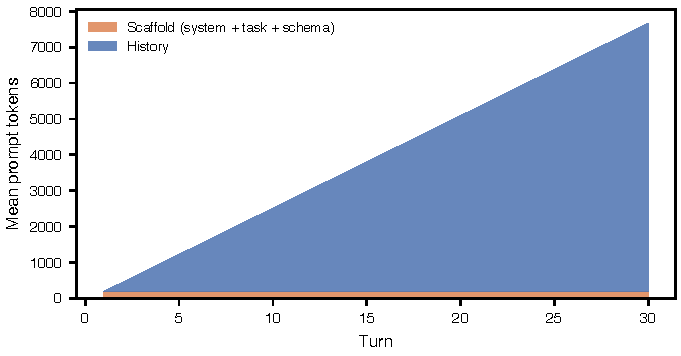
\includegraphics[width=\textwidth]{Fig1.pdf}
\caption{Stacked mean prompt tokens by region across agent turns (RTK off, compaction off, $n=12$ runs). Scaffold (system, task, and tool schema) is constant at 189 tokens; history accumulates above it at a mean rate of 258 tokens per turn.}
\label{fig:anatomy}
\end{figure}

\section{Taxonomy of Interventions}
\label{sec:taxonomy}

Prior survey-style treatments of this space organize by technique family: retrieval-based, compression-based, training-based. We organize by \emph{intervention point}---the moment in the agent execution loop at which the method acts. This choice is motivated by the recurrence analysis in Section~\ref{sec:background}: methods with the same intervention point share the same recurrence profile, and the interaction between two methods depends on whether they act on the same token population.

Methods are assigned to the earliest lifecycle point at which they directly modify serialized content or generation policy. Methods with distinct direct intervention points receive a hybrid label, while downstream effects on later token populations or trajectory length are recorded as secondary effects. Category~5 is reserved for explicit policy-level interventions before generation rather than serving as a residual category.

We define five intervention points:
\begin{enumerate}
\item \textbf{Pre-request schema provisioning} acts before the model receives any content for the current turn, by controlling which tool schemas are included in $B_t$. Population: schema tokens, recurring.
\item \textbf{Pre-context output filtering} acts at the tool-execution boundary, before tool output enters the conversation. Population: tool-result tokens, recurring.
\item \textbf{Post-hoc context compression} acts on content already present in the context, reducing its representation. Population: any prior content, recurring.
\item \textbf{Generation-time reasoning compression} modifies or constrains the tokens the model generates. Population: assistant-generated tokens $A_i$, which enter later prompt history only if retained.
\item \textbf{Pre-generation behavioral intervention} modifies the model's behavioral policy before generation, reducing unnecessary output. Population: generated content and trajectory behavior; effects may propagate through later tool calls and turn count $T$.
\end{enumerate}

Fig.~\ref{fig:taxonomy} schematizes the five intervention points along the agent execution loop. Table~\ref{tab:taxonomy} classifies sixteen methods across eight axes; karpathy-skills is included for taxonomy coverage but excluded from the quantitative arguments supporting C2 and C3 because it reports no numerical evaluation. Category~4 also includes CtrlCoT~\citep{ctrlcot2026}, Extra-CoT~\citep{extracot2026}, and SEER~\citep{seer2025}, which progressively increase training cost to achieve stable compression at extreme ratios. Every cell is sourced from the primary paper, repository README, or vendor documentation as indicated; self-reported values are marked~$^{\mathrm{a}}$. When a method family has multiple published versions, we include the most recent representative entry that satisfies our inclusion criteria; LLMLingua-2~\citep{llmlingua2} represents the LLMLingua line rather than LLMLingua-1, which it supersedes for task-agnostic prompt compression. TokenSkip~\citep{tokenskip2025} uses LLMLingua-2~\citep{llmlingua2} as its token-importance scoring component during training data generation---the only documented instance in the corpus of a Category~4 method depending on a Category~3 method, though this dependency is not evaluated as a composition.

\begin{figure}[htbp]
\centering
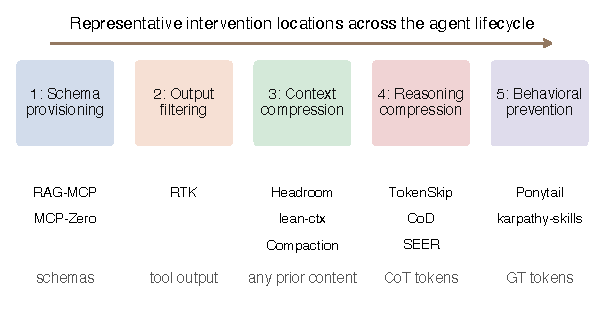
\includegraphics[width=\textwidth]{Fig2.pdf}
\caption{Schematic of five intervention points in the agent token lifecycle, with representative methods per category (not exhaustive; Table~\ref{tab:taxonomy} lists all sixteen). Labels below each category denote token populations; the arrow indicates representative intervention locations across the lifecycle, not a mandatory sequential pipeline.}
\label{fig:taxonomy}
\end{figure}

\begin{sidewaystable}[p]
\caption{Taxonomy of token-efficiency interventions by intervention point. PT = prompt tokens; GT = generated tokens. Evidence: P = peer-reviewed; A = arXiv preprint; S = self-reported. Cross-cat.\ records broader cross-category relations, including dependencies and baselines; Boolean cross-composition evidence is reported separately in Section~\ref{sec:claims}.}
\label{tab:taxonomy}
\centering
\footnotesize
\setlength{\tabcolsep}{3.5pt}
\renewcommand{\arraystretch}{1.18}
\begin{tabularx}{\textwidth}{@{}
  >{\raggedright\arraybackslash}p{1.85cm}
  >{\centering\arraybackslash}p{0.55cm}
  >{\raggedright\arraybackslash}p{1.45cm}
  >{\raggedright\arraybackslash}p{2.05cm}
  >{\centering\arraybackslash}p{1.05cm}
  >{\centering\arraybackslash}p{1.25cm}
  >{\centering\arraybackslash}p{0.55cm}
  >{\raggedright\arraybackslash}p{1.35cm}
  >{\raggedright\arraybackslash}X
@{}}
\toprule
Method & Cat. & Token pop. & Primary metric & Train & Access & Evid. & Cross-cat. & Failure mode \\
\midrule
RAG-MCP & 1 & schemas & selection acc.\ + PT & none & black-box & A & no & retrieval miss \\
MCP-Zero & 1 & schemas & selection acc.\ + avg PT & none & black-box & A & no & request quality \\
\tabtworow{RTK$^{\mathrm{a}}$}{\citep{rtk2024}} & 2 & tool output & estimated PT & none & black-box & S & no & silent omission \\
\tabtworow{Headroom$^{\mathrm{a}}$}{\citep{headroom2025}} & 3 & \shortstack[l]{tool output,\\history} & PT by content type & pretrained & black-box & S & no & handle loss at compaction \\
\tabtworow{lean-ctx$^{\mathrm{a}}$}{\citep{leancxt2025}} & 2/3 & \shortstack[l]{reads, shell,\\proxy} & PT by lang./mode & local learn & black-box & S & no & double compression \\
\tabtworow{Native comp.$^{\mathrm{a}}$}{\citep{nativecompaction2025}} & 3 & history & session continuation & none & black-box & S & no & summary info loss \\
TokenSkip & 4 & CoT & acc.\ vs ratio (math) & LoRA & white-box & P & Cat3 labeler & domain fragility \\
CtrlCoT & 4 & CoT & acc.\ vs ratio (math) & SFT & white-box & A & no & budget slack \\
Extra-CoT & 4 & CoT & acc.\ vs ratio (math) & SFT+RL & white-box & A & Cat3 baseline & training cost \\
Chain of Draft & 4 & CoT & acc.\ + GT + latency & none & black-box & A & no & zero-shot collapse \\
SEER & 4 & CoT & pass@1 + length + loops & SFT & white-box & A & no & single-model eval \\
Ponytail$^{\mathrm{a}}$ & 5 & code + session & LOC + session PT + cost & none & black-box & S & no & prompt-layer contention \\
\tabtworow{karpathy-skills$^{\mathrm{a}}$}{\citep{karpathy2025skills}} & 5 & behavior & none reported & none & black-box & S & no & deliberation inflation \\
LLMLingua-2 & 3 & any prompt text & QA F1 / BERTScore & pretrained & black-box & P & Cat4 labeler & silent loss \\
MemGPT & OUT & paging & task capability & none & white-box & A & internal stack & out of scope \\
Latent CoT & OUT & hidden state & acc.\ + latency & custom train & white-box & A & n/a & incommensurable unit \\
\bottomrule
\end{tabularx}
\footnotetext[a]{Self-reported or vendor documentation; not independently peer-reviewed.}
\footnotetext{Cat.\ = intervention-point category (Section~\ref{sec:taxonomy}). OUT = excluded boundary case (Section~\ref{sec:background}).}
\footnotetext{Failure modes include reported and analytically inferred risks; provenance is provided in the extraction sheet.}
\end{sidewaystable}

The intervention-point axis is a coding of each method's \emph{primary} action, not a claim that methods act at a single point. Several recent methods deliberately span points within one system: ACON~\citep{acon2025} jointly compresses tool observations (Category~2) and interaction history (Category~3); AgentDiet~\citep{agentdiet2025} prunes both across the trajectory and reports cost on all runs versus resolved-only runs; and LightThinker++~\citep{lightthinkerpp2026} couples reasoning compression (Category~4) with adaptive memory management (Category~3-like) in agentic tasks. We record these as category-spanning single methods rather than as cross-category \emph{compositions} in the sense of Section~\ref{sec:claims}, because each is one integrated method with one baseline rather than two separately baselined methods activated together. They nonetheless show that the boundaries this taxonomy draws are increasingly crossed inside individual methods, which is part of why a principled composition protocol is needed.

\section{Three Structural Claims}
\label{sec:claims}

Each claim is stated as a falsifiable claim supported by specific evidence from Table~\ref{tab:taxonomy} and cited sources.

\begin{table}[!htbp]
\caption{Per-method evaluation scope supporting claim C1 for the fourteen in-scope methods (MemGPT and Latent CoT excluded; Section~\ref{sec:background}). ``Cross-composed'' indicates whether the method has been evaluated in combination with any method from a different intervention-point category.}
\label{tab:c1_evidence}
\centering
\footnotesize
\begin{tabularx}{\textwidth}{@{}>{\raggedright\arraybackslash}p{3.3cm}c>{\raggedright\arraybackslash}X>{\raggedright\arraybackslash}X@{}}
\toprule
Method & Category & Evaluation setting & Cross-composed \\
\midrule
RAG-MCP & 1 & MCPBench WebSearch, 20 trials & No \\
MCP-Zero & 1 & APIBank multi-turn, 308 servers & No \\
RTK~\citep{rtk2024} & 2 & Self-reported session estimates & No \\
Headroom~\citep{headroom2025} & 3 & Self-reported content-type benchmarks & No \\
lean-ctx~\citep{leancxt2025} & 2/3 & Self-reported read/shell modes & No \\
Native compaction~\citep{nativecompaction2025} & 3 & Vendor mechanism docs, no benchmark & No \\
TokenSkip & 4 & GSM8K/MATH-500 single-shot & No (uses LLMLingua-2 as labeler only) \\
CtrlCoT & 4 & GSM8K/MATH-500 single-shot & No \\
Extra-CoT & 4 & Math CoT, single-shot & No \\
Chain of Draft & 4 & GSM8K/BIG-bench few-shot & No \\
SEER & 4 & Code/defect/search tasks & No \\
Ponytail & 5 & 12 feature tasks, 4 arms & No (same-slot ablation) \\
karpathy-skills~\citep{karpathy2025skills} & 5 & None reported & No \\
LLMLingua-2 & 3 & MeetingBank QA/summarization & No \\
\bottomrule
\end{tabularx}
\end{table}

\subsection{Claim C1: No Cross-Category Evaluation in the Corpus}

An evaluation crosses category boundaries if and only if two methods from different intervention-point categories are activated simultaneously and their combined effect is measured against individual baselines, where ``simultaneously'' means within a single agent trajectory.

The research corpus consists of papers and preprints retrieved through a structured search of arXiv (cs.LG, cs.CL, cs.AI), ACL Anthology, and IEEE Xplore using the queries ``LLM agent token efficiency,'' ``prompt compression agent,'' ``context window management LLM,'' and ``chain-of-thought compression,'' with final search date July 2026. We supplemented this corpus with backward citation tracing from included papers and removed duplicate records before coding. Grey literature (blog posts, technical reports, GitHub repositories, vendor documentation) was added for method identification and evaluation-scope coding. C1 applies to the combined defined corpus; rows in Table~\ref{tab:c1_evidence} reflect evidence type as denoted by the Evidence column in Table~\ref{tab:taxonomy} (P = peer-reviewed; A = arXiv preprint; S = self-reported or vendor documentation). The sixteen methods included satisfy at least one of: (a) at least one quantitative token-cost claim is made in the primary source, or (b) the method is publicly deployed or documented in practitioner-facing agent systems and is cited or discussed in the research corpus. karpathy-skills satisfies criterion (b) only and reports no quantitative metric, as noted in Table~\ref{tab:taxonomy}. Criterion (b) is used only for taxonomy coverage and does not confer quantitative evidentiary status.

We identified no cross-category composition evaluation, in the strict sense of two separate methods from different intervention-point categories activated together and measured against individual baselines, in the combined defined corpus. Table~\ref{tab:c1_evidence} records the Boolean cross-composed coding used for this claim; Table~\ref{tab:taxonomy}'s ``Cross-cat.'' column denotes broader cross-category relations and is not the C1 evidence field. The TokenSkip--LLMLingua-2 dependency noted in Section~\ref{sec:taxonomy} does not constitute a cross-category evaluation because LLMLingua-2 is used as an off-policy labeler during training data generation, not as a simultaneously active intervention during the evaluation trajectory.

We state the limits of this claim plainly, because it is narrower than a headline gap. First, a growing number of \emph{single} methods now span intervention-point categories internally: ACON~\citep{acon2025} combines observation compression (Category~2) with history management (Category~3), and AgentDiet~\citep{agentdiet2025} reduces trajectory content across both, reporting cost on all runs versus resolved-only runs. LightThinker++~\citep{lightthinkerpp2026}, which predates our hypothesis freeze, pairs reasoning compression (Category~4) with adaptive memory management (Category~3-like) in agentic tasks; it is genuine prior art for category-spanning behavior that our original corpus missed. These do not falsify C1's strict Boolean, since none composes two \emph{separate} baselined methods, but they show that the boundary C1 draws is increasingly crossed within individual methods, so the claim's significance is as motivation for a composition protocol, not as a standalone finding. Second, corpus search, deduplication, and screening counts were not systematically logged and coding was done by a single researcher; C1 is therefore limited to the final coded corpus and is not an exhaustive absence claim over the full literature.

\subsection{Claim C2: Published Evaluations Are Not Directly Commensurable}

Two interventions are directly commensurable in this context only if their reported results share a common token outcome, quality constraint, success denominator, and trajectory evaluation horizon, such that their ratio can be interpreted as relative session-level efficiency. In the final coded corpus, no pair of methods reports outcomes on all four dimensions simultaneously. Table~\ref{tab:c2} illustrates the gap: Category~1 methods report selection accuracy and prompt tokens on agent tool-selection tasks; Category~4 methods report math accuracy at compression ratio on single-shot reasoning benchmarks; Category~5 reports lines of code, session tokens, cost, and time on coding-agent tasks. This is not merely a reporting convention: under currently published evidence, cross-category composition cannot be evaluated from headline numbers alone, even before interaction effects are considered.

\begin{table}[!htbp]
\caption{Primary reported metrics, illustrating that no common evaluation protocol spans the defined corpus.}
\label{tab:c2}
\centering
\footnotesize
\begin{tabularx}{\textwidth}{@{}clX@{}}
\toprule
Cat. & Method & Primary reported metric \\
\midrule
1 & RAG-MCP & selection accuracy + prompt tokens (20 trials) \\
1 & MCP-Zero & selection accuracy + avg tokens \\
\midrule
2 & RTK (Rust Token Killer) & estimated tokens, no quality metric \\
\midrule
3 & Headroom & tokens by content type, ``same answers'' asserted \\
3 & lean-ctx / LeanCTX & tokens by language/mode \\
3 & Native compaction & session continuation, no published metric \\
3 & LLMLingua-2 & QA F1/BERTScore at ratio \\
\midrule
4 & TokenSkip & math accuracy vs compression ratio \\
4 & CtrlCoT & math accuracy vs compression ratio \\
4 & Extra-CoT & math accuracy vs compression ratio \\
4 & Chain of Draft (CoD) & accuracy + output tokens + latency \\
4 & SEER & pass@1 + CoT length + loop rate \\
\midrule
5 & Ponytail & LOC + session tokens + cost + time + safety rate \\
\bottomrule
\end{tabularx}
\end{table}

\subsection{Claim C3: Token Savings Exhibit Asymmetric Recurrence}

This follows analytically from the budget model in Section~\ref{sec:background}. Under full retention, a saving of $\Delta A_k$ or $\Delta O_k$ tokens at turn $k$ amplifies to $\Delta A_k \times (T-k)$ or $\Delta O_k \times (T-k)$ accumulated PT savings by session end. A saving of $\Delta S$ to scaffolding amplifies to $\Delta S \times T$. Category~4 primarily reduces $A_k$, which reduces future history; Category~5 may alter generated content, downstream tool output, and total trajectory length; Category~1 reduces $S$, which recurs at every turn; Category~2 reduces $O_k$, which also enters history and recurs.

Most quantitative methods report single-turn, single-task, or method-specific session outcomes. Such framing understates session-level savings for Categories~1 and~2, can overstate the recurring prompt-token value of late or unretained Category~4 savings (since GT savings at late turns have little recurrence remaining), and omits interaction effects across categories. Fig.~\ref{fig:c4} illustrates this asymmetry under three retention scenarios; it is a counterfactual illustration derived from~\eqref{eq:recurrence_ratio}, not an experimental result.

\begin{figure}[htbp]
\centering
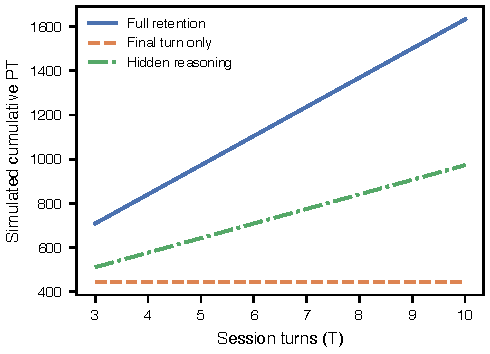
\includegraphics[width=\textwidth]{Fig3.pdf}
\caption{Simulated cumulative prompt tokens under a TokenSkip-like compression profile (313$\rightarrow$181 generated tokens per reasoning step, $\gamma{=}0.42$; based on published aggregate values from TokenSkip, not a reproduced run) across session lengths $T$. \emph{Full retention}: saved reasoning re-enters every later prompt. \emph{Final turn only}: the saving appears only in the final response. \emph{Hidden reasoning}: reasoning never enters subsequent prompts. Counterfactual illustration derived from~\eqref{eq:recurrence_ratio}, not an experimental result.}
\label{fig:c4}
\end{figure}

\section{Composition Study}
\label{sec:composition}

\subsection{Motivation}

C1 documents that none of the fourteen in-scope interventions in the final coded corpus had been evaluated in cross-category combination. This section reports two preregistered pilot evaluations---the first identified in the defined corpus---using a formal $2\times2$ factorial design. The choice of category pairs is theory-driven:

\textbf{E1 (RTK-compaction, Category~2 $\times$ Category~3):} Two mechanisms predict opposite interaction directions. RTK may reduce tool-output accumulation and delay the first compaction event; if this both lowers replayed tool output and avoids an otherwise costly or lossy compaction event, the combined arm may use fewer cumulative prompt tokens than the additive prediction, producing superadditive savings ($\hat{\Delta}<0$). Alternatively, if compaction already incorporates RTK-filtered output, the marginal gain from RTK under compaction is reduced, predicting sub-additivity ($\hat{\Delta}>0$). The preregistered direction is negative, driven by the delayed-trigger mechanism as the primary theoretical prediction.

\textbf{E2 (RTK-CoD, Category~2 $\times$ Category~4):} RTK acts directly on tool-output tokens $O_i$, whereas CoD acts directly on assistant-generated reasoning tokens $A_i$. Because cumulative GT is directly targeted only by CoD, E2 does not test the addition of two direct GT-reduction mechanisms. Instead, it tests whether RTK modifies CoD's cumulative-GT effect indirectly through changed observations, tool-use patterns, retries, or trajectory length. Under unchanged trajectories, the preregistered prediction is a near-zero interaction on cumulative GT.

These pilots cover two of the ten possible cross-category pairs and are intended to demonstrate the evaluation protocol and examine two theoretically distinct interaction regimes, not to validate predictions across the full taxonomy.

\subsection{Experimental Design}

The agent runs Qwen2.5-Coder-7B-Instruct (HuggingFace revision c03e6d358207e414f1eca0bb1891e29f1db0e242) served with vLLM~0.8.5 on a single NVIDIA A40 (48~GB), prefix caching enabled, at temperature~0.2 and top-$p$~0.95. We use temperature~0.2 rather than greedy decoding so that repeated seeds probe genuine trajectory variability; Section~\ref{sec:composition} reports how little diversity this actually produced. The task suite is six single-file Python bug-fix fixtures, each a source file with one deliberate logic error and a pytest suite the agent must make pass, constructed to be solvable in three to ten turns under correct behavior, with a hard stop at 30 turns. This narrow, controlled task family is a deliberate choice for a measurement study: it keeps everything except the interventions fixed, so that any residual variance is a property of the agent and the outcome rather than of task heterogeneity.

The three interventions instantiate three of the taxonomy's categories. Output filtering (Category~2), realized as RTK, is a Rust binary that intercepts shell tool calls and compresses command output before it enters context. Compaction (Category~3) is a threshold-triggered summarizer that fires when occupancy $B_t$ exceeds $\tau=4{,}096$ tokens, summarizing with the same model at temperature~0.0. Reasoning compression (Category~4) is Chain of Draft~\citep{chainofdraft2025}, a system-prompt instruction constraining each reasoning step to five words.

We ran two factorial experiments chosen for theoretically distinct interaction regimes. The primary experiment, E1, crosses output filtering with compaction (RTK $\in\{\text{off},\text{on}\}$ $\times$ compaction $\in\{\text{off},\text{on}\}$) over six tasks and two seeds, giving $n=12$ per cell and 48 runs; its outcome is cumulative serialized prompt tokens $\mathrm{PT}_{\mathrm{cum}}=\sum_t B_t$, the exact quantity these two categories act on. The secondary experiment, E2, crosses output filtering with reasoning compression over six tasks and six seeds ($n=36$ per cell, 144 runs) with cumulative generated tokens $\mathrm{GT}_{\mathrm{cum}}=\sum_t \mathrm{GT}_t$ as its outcome. E1 used the two confirmatory seeds (17, 52) fixed in its hypothesis file; E2 used six seeds (7, 13, 17, 42, 52, 99), fixed in \texttt{e1b\_frozen.yaml} (Appendix~\ref{app:prereg}) before E2 data collection as a deliberate replication decision rather than a post-hoc change. Hypothesis direction, statistical model, primary estimand, and analysis code were committed and SHA-256 hashed before data collection (Appendix~\ref{app:prereg}); the confirmatory estimands reproduce byte-for-byte from the raw run traces through the archived pipeline (Section~\ref{sec:composition}). We designate E1 the primary experiment on process-integrity grounds decided before outcomes were examined: E1 has no process-degenerate runs and retains all six tasks in every cell, whereas E2's degeneracy loads on the reasoning-compression arms, so filtering E2 to recover its interaction would condition on a treatment-induced collider (Section~\ref{sec:composition}).

Matplotlib figure scripts were drafted with assistance from ChatGPT (OpenAI); all figure code was reviewed, edited, and executed by the authors, who take full responsibility for the published plots.

The preregistered estimand is the raw interaction
\begin{equation}
  \hat{\Delta} = Y_{11} - Y_{10} - Y_{01} + Y_{00}
  \label{eq:interaction}
\end{equation}
where $Y_{ab}$ denotes the cell mean for RTK$=a$ and the second factor$=b$, $a,b\in\{0,1\}$. Negative $\hat{\Delta}$ indicates superadditive savings (combined saving exceeds the sum of parts); zero indicates additivity on the raw outcome scale; positive indicates sub-additivity. The preregistered direction for E1 is $\hat{\Delta}<0$.

A scale-free secondary estimand is
\begin{equation}
  \hat{\Delta}_{\log} = \log Y_{11} - \log Y_{10} - \log Y_{01} + \log Y_{00}.
  \label{eq:log_interaction}
\end{equation}
E1 observed value: $\hat{\Delta}_{\log}=+0.026$, numerically close to zero.

The statistical model is
\begin{align}
  Y_i &= \alpha
          + \beta_1 \cdot \mathrm{RTK}_i
          + \beta_2 \cdot \mathrm{Factor}_i
          + \beta_3 \cdot (\mathrm{RTK}_i \times \mathrm{Factor}_i) \nonumber\\
      &\quad + \sum_{k=1}^{K-1} \gamma_k \cdot \mathbf{1}[\mathrm{task}(i)=k]
          + \sum_{\ell=2}^{L} \delta_\ell \cdot s_{i\ell}
          + \varepsilon_i
  \label{eq:ols}
\end{align}
where $Y_i=\mathrm{PT}_{\mathrm{cum},i}$ in E1 and $Y_i=\mathrm{GT}_{\mathrm{cum},i}$ in E2. There are $K=6$ task levels, represented by $K{-}1=5$ fixed-effect indicators; $\varepsilon_i$ is the residual. For E1, $L=2$ and $s_{i2}\in\{0,1\}$ is a binary indicator for seed 52 vs.\ 17. For E2, $L=6$ and seed enters as five categorical fixed effects (one indicator per seed against a reference). The block-bootstrap resamples at the (task, seed) block level in both cases. Confidence intervals use block bootstrap with $B=1{,}000$ resamples:
\begin{equation}
  \hat{\Delta}^{*(b)} = Y_{11}^{*(b)} - Y_{10}^{*(b)} - Y_{01}^{*(b)} + Y_{00}^{*(b)}.
  \label{eq:bootstrap}
\end{equation}

\textbf{Precision:} The observed standard error, $\mathrm{SE}(\hat{\Delta})=28{,}755$ PT, implies a detectable interaction magnitude of approximately 80{,}514 cumulative PT under a normal approximation at 80\% power. The 95\% bootstrap CI $[-46{,}984,\;+50{,}141]$ communicates the precision more directly: interactions outside that range are incompatible with the data under the stated block-bootstrap procedure; moderate effects in either direction remain undetectable at this sample size.

\subsection{Results}

\textbf{Treatment delivery:} Of the 24 compaction-on runs in E1, 10 triggered at least one compaction event (activation rate 41.7\%, 5/12 per RTK level). Results below include all 24 runs regardless of activation, consistent with intent-to-treat analysis.

Table~\ref{tab:e1_results} and Fig.~\ref{fig:e1_cells} report E1 cell means. The confidence interval $[-46{,}984,\;+50{,}141]$~PT includes zero and spans substantial positive and negative interactions ($\hat{\Delta}=+2{,}897$~PT). The ordinary least squares (OLS) estimate of the interaction coefficient is $\hat{\beta}_3=+2{,}897$ ($\mathrm{SE}=28{,}755$); $R^2=0.185$. The preregistered direction (negative) is not supported.

For E2 (RTK-CoD), $\hat{\Delta}=-5.06$~GT (95\% CI $[-407,\;+374]$; $R^2=0.355$). Fig.~\ref{fig:e1b_cells} shows the interaction plot. Observed marginal differences were approximately $-124$~GT for RTK $\bigl(\tfrac{Y_{10}+Y_{11}}{2} - \tfrac{Y_{00}+Y_{01}}{2}\bigr)$ and $-126$~GT for CoD $\bigl(\tfrac{Y_{01}+Y_{11}}{2} - \tfrac{Y_{00}+Y_{10}}{2}\bigr)$; confidence intervals were not computed for these descriptive contrasts. The point estimate is numerically close to zero and aligned with the preregistered prediction that RTK would not materially modify CoD's cumulative-GT effect under unchanged trajectories, but the confidence interval is too wide to establish equivalence.

We report a per-success cost that the recent efficiency-evaluation literature calls \emph{cost-of-pass}~\citep{costofpass2025}, the ratio of total cost to number of successes $v=C/R$. This is the same quantity an earlier draft of this work named ``success-adjusted cost''; we adopt the established term. With cumulative prompt tokens as the cost, the per-cell cost-of-pass is
\begin{equation}
  v(c)
  = \frac{\displaystyle\sum_{i \in c} \mathrm{PT}_{\mathrm{cum},i}}{\displaystyle\sum_{i \in c} \mathbf{1}[\mathrm{success}_i]}.
  \label{eq:sac}
\end{equation}
Cost-of-pass is a descriptive secondary statistic here; no hypothesis was preregistered on it, and it is used in agent-efficiency evaluation precisely because token counts alone ignore whether the task was solved~\citep{costofpass2025, aiagentsmatter2024, efficientagents2025}. Fig.~\ref{fig:sac} shows $v(Y_{00})=245{,}527$ versus $v(Y_{11})=68{,}685$ prompt tokens per success; the former rests on only 3 successful runs out of 12 and is highly unstable. The bootstrapped CI for $v(Y_{00})$ is very wide and the point estimate should not be over-interpreted. The large differences are primarily attributable to differing success denominators and longer failed trajectories, not to per-turn token compression alone. Success was 9/12 with compaction and 3/12 without compaction in the RTK-off cells. A plausible mechanism, not proven by this design, is that compaction extends the agent's effective runway on long failing traces by preventing context exhaustion before the repair is found; failed runs in $Y_{00}$ therefore accumulate far more tokens before the 30-turn budget expires.

\begin{table}[!htbp]
\caption{E1 cell means and estimands. Outcome: cumulative serialized prompt tokens (PT). $v$ = cost-of-pass~\citep{costofpass2025}, prompt tokens per successful task completion (descriptive, not preregistered).}
\label{tab:e1_results}
\centering
\footnotesize
\setlength{\tabcolsep}{4pt}
\begin{tabularx}{\textwidth}{@{}llcXcc@{}}
\toprule
Cell & RTK & Compaction & Mean PT & Succ. & $v$ (cost-of-pass) \\
\midrule
$Y_{00}$ & off & off & 61{,}382 & 3/12 & 245{,}527 \\
$Y_{01}$ & off & on  & 36{,}438 & 9/12 & 48{,}583 \\
$Y_{10}$ & on  & off & 56{,}389 & 4/12 & 169{,}168 \\
$Y_{11}$ & on  & on  & 34{,}343 & 6/12 & 68{,}685 \\
\midrule
\begin{minipage}[t]{1.1cm}\raggedright$\hat{\Delta}$\end{minipage} & \multicolumn{2}{c}{--} & 2{,}897 & -- & -- \\
95\% CI & \multicolumn{2}{c}{--} & $[-46{,}984,\;{+}50{,}141]$ & -- & -- \\
\bottomrule
\end{tabularx}
\footnotetext{$n=12$ per cell (6 tasks $\times$ 2 seeds). Model: Qwen2.5-Coder-7B-Instruct (rev.~c03e6d3). Compaction trigger $\tau=4{,}096$ tokens.}
\end{table}

\begin{figure}[htbp]
\centering
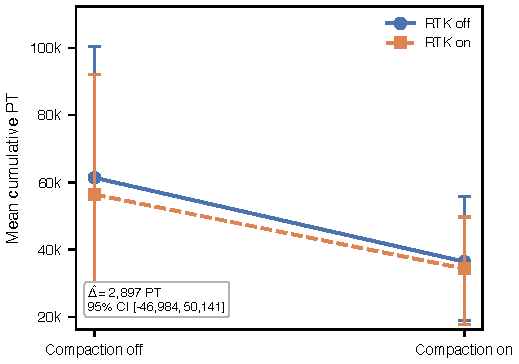
\includegraphics[width=\textwidth]{Fig4.pdf}
\caption{Mean cumulative PT per cell, E1 (RTK-compaction) experiment ($n=12$). Error bars show run-level bootstrap confidence intervals for individual cell means; the interaction interval uses the preregistered task-seed block bootstrap. Solid circles/blue: RTK off; dashed squares/orange: RTK on. Interaction $\hat{\Delta}=+2{,}897$~PT (95\% CI $[-46{,}984,\;+50{,}141]$).}
\label{fig:e1_cells}
\end{figure}

\begin{figure}[htbp]
\centering
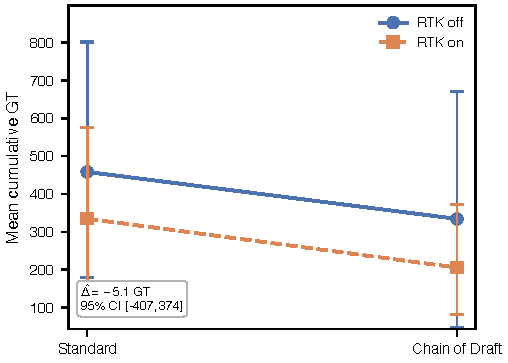
\includegraphics[width=\textwidth]{Fig5.pdf}
\caption{Mean cumulative GT per cell, E2 (RTK-CoD) experiment ($n=36$). Error bars show run-level bootstrap confidence intervals for individual cell means; the interaction interval uses the preregistered task-seed block bootstrap. Solid/dashed lines: RTK off/on. Interaction $\hat{\Delta}=-5.06$~GT (95\% CI $[-407,\;+374]$). Observed marginal differences: RTK $\approx -124$~GT; CoD $\approx -126$~GT (descriptive contrasts; no CIs).}
\label{fig:e1b_cells}
\end{figure}

\begin{figure}[htbp]
\centering
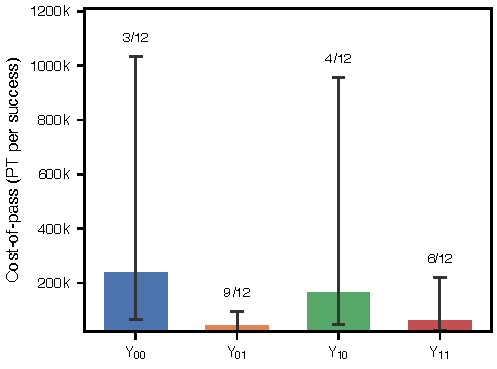
\includegraphics[width=\textwidth]{Fig6.pdf}
\caption{Cost-of-pass~\citep{costofpass2025} (prompt tokens per successful task completion) by treatment cell, E1 experiment. Error bars show run-level bootstrap intervals for descriptive estimates; bootstrap replicates with zero successful runs were undefined and omitted. Success counts are shown above each bar. Descriptive secondary analysis, not a preregistered confirmatory result.}
\label{fig:sac}
\end{figure}

\subsection{Measurement Audit}
\label{sec:audit}

The primary estimand is one contrast among many the design can express. To characterize what the experiment can and cannot detect, we computed every token-outcome contrast E1 supports: the two treatment main effects and their interaction, each on six outcomes (cumulative prompt tokens, cumulative generated tokens, their per-turn forms, turn count, and total tool-output tokens). Each is estimated with the preregistered task-seed block bootstrap ($B=1{,}000$, resampling the twelve (task, seed) blocks), which yields the point estimate, a bootstrap standard error, and a 95\% interval on the same footing as the primary analysis. Table~\ref{tab:audit} is the result and is the paper's central exhibit.

\begin{table}[!htbp]
\caption{Measurement audit of E1: every token-outcome contrast, with task-seed block-bootstrap standard error and 95\% interval. ``Det.'' marks whether the 95\% interval excludes zero. Only three of eighteen contrasts are distinguishable from zero, and all three are treatment-fidelity checks (output filtering reduces tool output; compaction reduces prompt tokens, in raw and per-turn form). No compositional (interaction) or downstream contrast is detectable. None of the three survives multiplicity correction (Bonferroni $\alpha=0.0028$ needs $|t|\gtrsim2.98$); under the correct $t(11)$ reference the raw compaction$\rightarrow$PT effect ($|t|=2.08$) does not clear even the uncorrected threshold of $2.201$.}
\label{tab:audit}
\centering
\footnotesize
\setlength{\tabcolsep}{4pt}
\begin{tabularx}{\textwidth}{@{}llrrrXc@{}}
\toprule
Contrast & Outcome & Estimate & SE & $|t|$ & 95\% CI & Det. \\
\midrule
RTK main & tool output & $-803$ & $356$ & $2.26$ & $[-1{,}539,\;-145]$ & yes \\
RTK main & PT & $-3{,}544$ & $13{,}588$ & $0.26$ & $[-28{,}419,\;+22{,}808]$ & no \\
RTK main & PT/turn & $-142$ & $387$ & $0.37$ & $[-859,\;+632]$ & no \\
RTK main & GT & $+11$ & $715$ & $0.02$ & $[-1{,}386,\;+1{,}326]$ & no \\
RTK main & GT/turn & $+2.4$ & $20.4$ & $0.12$ & $[-40.5,\;+36.6]$ & no \\
RTK main & turns & $+0.33$ & $3.07$ & $0.11$ & $[-5.9,\;+5.8]$ & no \\
\midrule
Compaction main & PT & $-23{,}495$ & $11{,}307$ & $2.08$ & $[-45{,}964,\;-2{,}603]$ & yes \\
Compaction main & PT/turn & $-774$ & $324$ & $2.39$ & $[-1{,}440,\;-163]$ & yes \\
Compaction main & GT & $-362$ & $494$ & $0.73$ & $[-1{,}355,\;+639]$ & no \\
Compaction main & GT/turn & $-3.8$ & $10.5$ & $0.37$ & $[-21.7,\;+17.8]$ & no \\
Compaction main & turns & $-0.58$ & $2.57$ & $0.23$ & $[-5.5,\;+4.5]$ & no \\
Compaction main & tool output & $-464$ & $470$ & $0.99$ & $[-1{,}360,\;+458]$ & no \\
\midrule
Interaction & PT & $+2{,}898$ & $25{,}673$ & $0.11$ & $[-46{,}984,\;+50{,}141]$ & no \\
Interaction & PT/turn & $+90$ & $797$ & $0.11$ & $[-1{,}467,\;+1{,}582]$ & no \\
Interaction & GT & $-1{,}923$ & $1{,}544$ & $1.25$ & $[-4{,}838,\;+1{,}027]$ & no \\
Interaction & GT/turn & $-78.6$ & $43.5$ & $1.80$ & $[-161,\;+3.8]$ & no \\
Interaction & turns & $+1.3$ & $5.3$ & $0.25$ & $[-8.3,\;+12.2]$ & no \\
Interaction & tool output & $+859$ & $898$ & $0.96$ & $[-876,\;+2{,}487]$ & no \\
\bottomrule
\end{tabularx}
\footnotetext{$n=12$ per cell, twelve (task, seed) blocks. PT/turn and PT for compaction are the same effect in different units and are not independent tests.}
\end{table}

\textbf{The survivors are manipulation checks, not findings.} The three detectable contrasts are exactly the two mechanical effects each treatment is defined to produce, one appearing in both raw and per-turn units. Output filtering reduces tool output because compressing tool output is what it does; compaction reduces prompt tokens because summarizing history is what it does. These are treatment-fidelity checks: they confirm the interventions were delivered, not that anything was discovered. The honest one-line summary of the audit is therefore \emph{treatment fidelity is confirmed, and no compositional or downstream effect is detectable}.

\textbf{Even the fidelity checks are marginal, and that is the point.} With eighteen contrasts at $\alpha=0.05$ one expects roughly $0.9$ false positives; three are detected, but none survives a Bonferroni correction, which requires $|t|\gtrsim2.98$. Under the correct reference distribution for twelve blocks, $t(11)$ with two-sided critical value $2.201$, the raw compaction$\rightarrow$PT effect ($|t|=2.08$) does not clear even the uncorrected threshold, and the block bootstrap over only twelve blocks is anti-conservative, so these marginal cases are where that bites hardest. A manipulation check ought to be overwhelming. Output filtering halves tool output, from a mean of $1{,}603$ to $800$ tokens, and this most direct effect in the entire design still reaches only $|t|=2.26$. When a design can barely detect its own manipulation, it cannot detect a second-order interaction between two manipulations. That is the paper's thesis, demonstrated at the strongest available point in the data.

\textbf{A falsifiable prediction, tested and inconclusive.} The accounting framework makes an a priori prediction here: a measured tool-output reduction should propagate to cumulative prompt tokens with the replay recurrence of Equation~\eqref{eq:toolout_savings}. Using the actual per-turn positions of the filtered output, that prediction is a saving of about $15{,}300$ prompt tokens under output filtering with compaction off. The observed effect is $-3{,}544$ with a 95\% interval of $[-28{,}419,\;+22{,}808]$. The prediction lies inside that interval, and so does zero. The test therefore cannot distinguish the model being correct, the model over-predicting, or output filtering having no net prompt-token effect at all. We report it as inconclusive rather than as either confirmation or refutation, because the target quantity is not resolvable at this sample size.

\textbf{What the measurement costs.} The binding constraint is the variance of cumulative prompt tokens, whose per-cell standard deviation ($\approx 62{,}700$) is about equal to its mean ($\approx 58{,}900$) because failed runs accumulate several times more tokens than successful ones. A standard two-sided power calculation at $80\%$ power then gives the sample sizes in Table~\ref{tab:power}. Resolving the prompt-token effect we actually observe would take roughly $4{,}900$ runs per cell; even the larger effect the accounting framework predicts would take about $265$. The experiment used twelve. This is the concrete price of doing this class of composition measurement to a standard that supports a claim, and it is the number a practitioner reporting a single-method saving without a power analysis is implicitly ignoring.

\begin{table}[!htbp]
\caption{Runs per cell required to detect an effect at $80\%$ power, two-sided $\alpha=0.05$, at the observed cumulative-token dispersion. The last row is the quantity the pilot actually observed.}
\label{tab:power}
\centering
\footnotesize
\begin{tabularx}{\textwidth}{@{}Xr@{}}
\toprule
Target effect & Runs/cell \\
\midrule
A $\approx$1{,}000-token generated-token effect (E2 scale) & $\approx 165$ \\
The accounting-framework-predicted output-filtering PT effect ($\approx$15{,}300) & $\approx 265$ \\
The observed output-filtering PT effect ($\approx$5{,}000) & $\approx 4{,}900$ \\
\bottomrule
\end{tabularx}
\footnotetext{Present design: $n=12$ per cell.}
\end{table}

\subsection{Interpretation}

The largest observed source of variation is task success/failure: runs in which the agent fails to repair the bug within the 30-turn budget accumulate 3--10$\times$ more tokens than successful runs. The interquartile range of cumulative PT across all 48 E1 runs spans approximately 69k--192k tokens, compared to a point estimate of 2,897. Separately from the interaction question, the success rates vary substantially across cells (3/12, 9/12, 4/12, 6/12 for $Y_{00}$, $Y_{01}$, $Y_{10}$, $Y_{11}$ respectively), suggesting a possible positive association between compaction and task completion in this sample---this observation is consistent with the cost-of-pass pattern but is not part of the preregistered confirmatory analysis on prompt tokens.

Two non-exclusive explanations are consistent with the near-zero interaction estimate and wide confidence interval. First, RTK reduces newly produced tool output, whereas compaction acts only after enough prior history has accumulated; the two mechanisms therefore operate on different parts of the trajectory. Second, \emph{insufficient power and low treatment fidelity}: with $n=12$ per cell, SE$(\hat{\Delta})=28{,}755$, and compaction activation in only 41.7\% of compaction-on runs, the 95\% CI is incompatible with interaction magnitudes outside $[-46{,}984,\;+50{,}141]$~PT under the stated block-bootstrap procedure, but is uninformative about smaller effects. This paper does not claim the interaction is zero; the interval includes zero and is too wide to resolve moderate interactions at this sample size.

\subsection{Evaluation Diagnostics}
\label{sec:diagnostics}

Two properties of the runs, orthogonal to the interaction question, are reusable lessons for anyone running agent evaluations at this scale.

\textbf{Process-based degeneracy.} Nominal run counts overstate information. We flag a run as process-degenerate if it makes no tool call, terminates at the first turn, or exactly duplicates the trajectory of another run in its cell; these are process criteria, applied without reference to the outcome. In E2, 104 of 144 runs (72.2\%) were degenerate. The flag is not distributed evenly: it loads on the reasoning-compression arms, 77.8\% under Chain of Draft versus 66.7\% without, in both output-filtering conditions, matching the zero-shot-collapse failure mode recorded for that method in Table~\ref{tab:taxonomy}. This is treatment-induced degeneracy, so it is a collider: filtering E2 down to its non-degenerate runs to sharpen the interaction would condition on a variable that the treatment causes, biasing the very estimate the filter was meant to clean. It is why we designate E1, which has no degenerate runs, the primary experiment, and report E2 descriptively. A process-based degeneracy audit of this kind is cheap and exposes how much of a nominal sample actually carries information.

\textbf{Seed expansion buys little at low temperature.} E2 used six random seeds per cell to E1's two, on the expectation that more seeds would proportionally increase trajectory diversity. At temperature 0.2 they did not: E1 averaged 2.0 distinct trajectories per cell from its two seeds, and E2 averaged 2.9 from its six. Tripling the seed count bought about one extra distinct trajectory. For a study of this kind, replication should come from adding tasks and task families, which move the dominant between-task variance component, rather than from adding seeds, which mostly reproduce trajectories the model already visited.

\section{Discussion}
\label{sec:discussion}

The two pilot experiments illustrate the evaluation protocol; they do not establish any compositional effect, and the measurement audit (Section~\ref{sec:audit}) explains why they could not. The value of the pilot is not the interaction point estimate but the audit it makes possible: a quantified account of what this class of composition measurement costs. An imprecise estimate is uninformative as a finding, but the reason it is imprecise, cumulative-token variance about equal to the mean, is itself a stable, reportable property of agent evaluation on this outcome. We frame the paper around that property rather than around the null it produces.

The distinction matters for how the result should be read. A pure null-result reading would claim that we looked for an interaction and found none, which invites the objection that absence of evidence is not evidence of absence, and which is in any case not quite what happened. We did not find no interaction; we found that this design could not have detected one, together with the sample size at which it could. That is a claim about the measurement, and unlike a claim about the interaction it is fully supported by the data in hand. The same lens reframes the two effects that are detectable: they are treatment-fidelity checks, so the design's ability to detect its own manipulations only barely, while failing to detect anything second-order, is direct evidence for the cost argument rather than a scattering of weak positive findings.

Concurrent work reaches compatible conclusions about the gap between token counts and end-to-end cost by complementary, non-analytic means. \citet{tokennotcost2026} decompose token change into per-turn and trajectory terms over paired blocks with provider-billed cost as the primary metric, on coding agents, and study output filtering specifically; that preprint appeared one day before our hypothesis freeze and could not have informed our preregistration. \citet{compressioncost2026} argue that completion metrics hide the interaction cost of compression and attribute reacquisition cost by paired counterfactual injection. Both measure the split post hoc; our framework instead derives the replay term a priori from the recurrence in Section~\ref{sec:background}, and we position the two lines as mutually corroborating rather than competing. Stronger compositional evidence would require the sample sizes of Table~\ref{tab:power} across additional category pairs, model families, and task types, with confirmed intervention activation and shared outcome definitions.

\textbf{Limitations:}
\begin{enumerate}
\item Single model family (Qwen2.5-Coder-7B-Instruct). Category~4 methods such as TokenSkip are trained-model interventions; our Chain of Draft implementation is a prompt-only approximation.
\item Single task domain (Python bug-fix, single-file). Harder tasks with longer successful trajectories might exhibit different compaction-trigger dynamics.
\item $n=12$ per E1 cell; $n=36$ per E2 cell. E1 is underpowered for interaction detection at small-to-moderate effect sizes.
\item Several category combinations remain untested, including all involving Category~1 or Category~5 and within-Category-3 compositions (compaction $\times$ context compression/retrieval methods).
\item The compaction implementation is a custom threshold-triggered summarizer, not Headroom, lean-ctx, or native Claude Code compaction specifically.
\item Corpus search, screening, and coding were conducted by a single researcher without independent dual screening, dual coding, or inter-rater reliability assessment. The C1 finding is bounded by the final coded corpus and the documented search procedure.
\end{enumerate}

\textbf{Research agenda:}
\begin{itemize}
\item \textbf{H1:} CCR-based compression handles (Headroom) do not survive compaction summary boundaries. Testable by running a joint CCR+compaction session and querying original content after a compaction event.
\item \textbf{H2:} Chain of Draft degrades tool-call planning accuracy in multi-step agentic tasks. Testable by measuring tool-call error rates under CoD vs.\ standard reasoning.
\item \textbf{H3:} Output filtering (RTK) delays compaction trigger events in proportion to tool-output compression ratio. Testable by comparing compaction event counts across RTK-compaction cells at fixed $\tau$.
\item \textbf{H4:} Schema retrieval (RAG-MCP) and reasoning compression (CoD) interact negatively on tool-selection accuracy. Testable in a $2\times2$ with tool-selection accuracy as the outcome.
\item \textbf{H5:} LLMLingua-2 applied to tool schemas reduces prompt tokens with no degradation to tool-selection accuracy. Testable with zero new training using the publicly available LLMLingua-2 model.
\end{itemize}

\section{Related Work}
\label{sec:related}

\textbf{Prompt and context compression:} Text-level prompt compression methods, exemplified by LLMLingua-2~\citep{llmlingua2}, reduce serialized prompt tokens on fixed inputs and are typically evaluated on QA or summarization benchmarks with F1 or BERTScore at a target compression ratio. Session-management approaches in our Category~3 (Headroom, lean-ctx, native compaction) instead target accumulated agent history and tool output across turns. Neither line reports cross-category composition with schema retrieval, output filtering, or reasoning compression, and their primary metrics differ from agent task-success rates used in Categories~1 and~5.

\textbf{Efficient reasoning and agent-efficiency evaluation:} Surveys and method papers on CoT efficiency~\citep{sui2025survey, tokenskip2025, chainofdraft2025, ctrlcot2026, extracot2026, seer2025} focus primarily on Category~4: accuracy versus generated-token reduction on mathematical reasoning tasks. A parallel line argues that token counts are the wrong unit for agent efficiency and that cost must be adjusted for success: cost-of-pass~\citep{costofpass2025} formalizes cost per solved instance, \citet{aiagentsmatter2024} document how unadjusted metrics mislead, and \citet{efficientagents2025} apply the resulting accuracy-cost view to agent design. Our cost-of-pass reporting (Section~\ref{sec:composition}) follows this line. Agent and software-engineering benchmarks increasingly report task completion, pass rates, and turn counts, but rarely standardize cumulative serialized prompt tokens, generated tokens, and intervention activation within a composable factorial design, and rarely report the power such a design would need. Our taxonomy, accounting framework, and measurement audit address that gap directly.

\textbf{Decomposing agent token cost:} Concurrent work decomposes agent token or cost change into per-turn and trajectory components empirically. \citet{tokennotcost2026} study output filtering on coding agents with a paired, provider-billed design and a success-adjusted end-to-end cost metric; \citet{compressioncost2026} attribute the interaction cost of compression through paired counterfactual state injection. These measure the split from data; our accounting framework derives the replay component a priori from the token-recurrence structure and then tests it against measurement, so the two approaches are complementary. We report our one such test as inconclusive at the pilot sample size (Section~\ref{sec:audit}).

\textbf{Agent memory:} MemGPT~\citep{memgpt2023} addresses context limitations through OS-inspired paging rather than compression. This is architecturally orthogonal---it extends the effective context rather than reducing per-turn cost---and is therefore excluded from the taxonomy scope (Section~\ref{sec:background}).

\section{Conclusion}
\label{sec:conclusion}

We systematize fourteen in-scope token-efficiency interventions (thirteen with reported evaluation evidence) by where they act in the agent lifecycle and formalize how their savings recur across turns in a common accounting framework. We then ask what it costs to measure whether these interventions compose, and answer it with a preregistered $2{\times}2$ pilot and a measurement audit. The audit is the paper's central result: across eighteen token-outcome contrasts only the treatment-fidelity checks are detectable, none survives multiplicity correction, no compositional or downstream effect is detectable, and resolving the effect we do observe would require thousands of runs per cell against the twelve used. Cumulative-token variance about equal to its mean, treatment-loaded process degeneracy, and the futility of seed expansion at low temperature are stable, reusable properties of this evaluation setting. The contribution is thus a taxonomy, an accounting framework, and a measured account of what evaluating composition costs, with the pilot as the worked example rather than as evidence that the interventions are independent. Five specific hypotheses remain untested and are proposed as a research agenda.

\backmatter

\section*{Statements and Declarations}

\subsection*{Funding}
The authors did not receive support from any organization for the submitted work.

\subsection*{Competing interests}
The authors have no relevant financial or non-financial interests to disclose.

\subsection*{Ethics approval and consent to participate}
Not applicable.

\subsection*{Consent for publication}
Not applicable.

\subsection*{Data availability}
Aggregated experimental results supporting the composition study, including the frozen preregistered hypothesis files whose SHA-256 hashes are listed in Appendix~\ref{app:prereg}, are archived at Zenodo, \url{https://doi.org/10.5281/zenodo.21715347}~\citep{cab_dataset2026}. Raw agent run traces are not publicly archived owing to their size and environment-specific paths; they are available from the corresponding author on reasonable request.

\subsection*{Materials availability}
Not applicable.

\subsection*{Code availability}
Analysis scripts, figure-generation code, and aggregated outputs are archived at Zenodo, \url{https://doi.org/10.5281/zenodo.21715347}~\citep{cab_dataset2026}. The confirmatory estimands and the full measurement audit of Section~\ref{sec:audit} reproduce byte-for-byte from the raw run traces through the archived extraction and bootstrap pipeline, whose preregistered hypothesis-file hashes are listed in Appendix~\ref{app:prereg}.

\subsection*{Author contributions}
Soumitra Mehrotra conceived the study, designed and conducted the experiments, performed the analysis, and wrote the manuscript. Shubhender Singh contributed to the taxonomy framing, reviewed the structural claims and composition-study interpretation, and revised the manuscript. Saurabh Aggarwal contributed to the related-work synthesis, reviewed the evidence-audit tables and experimental methodology, and revised the manuscript.

\begin{appendices}

\section{C1 Evidence Table}
\label{app:c1}

Table~\ref{tab:c1_evidence} (Section~\ref{sec:claims}) lists the baseline evaluation scope for the fourteen in-scope methods in the taxonomy (Table~\ref{tab:taxonomy}). MemGPT and Latent CoT are excluded boundary cases (Section~\ref{sec:background}) and appear only in Table~\ref{tab:taxonomy} as OUT entries. No in-scope row reports simultaneous activation of methods from different intervention-point categories within a single agent trajectory.

\section{Experimental Details}
\label{app:experimental}

\textbf{Model and serving:} Qwen2.5-Coder-7B-Instruct (revision c03e6d358207e414f1eca0bb1891e29f1db0e242), vLLM~0.8.5, single NVIDIA A40 (48~GB), bfloat16, max model length 32{,}768, prefix caching enabled. Generation: temperature~0.2, top-p~0.95, max tokens 2{,}048.

\textbf{Tasks:} Six single-file Python bug-fix fixtures (\texttt{repo\_task\_001}--\texttt{repo\_task\_006}). Each contains one deliberate logic error and a pytest suite. Maximum agent turns: 30. Hard stop occupancy: 16{,}384 tokens.

\textbf{RTK:} Rust binary intercepting shell tool calls; activated when \texttt{rtk=on}. Compaction: threshold $\tau=4{,}096$ serialized prompt tokens; summarizer uses the same model at temperature~0.0. Chain of Draft: system prompt instruction limiting each reasoning step to five words.

\textbf{Blocking:} E1 (RTK-compaction): 6 tasks $\times$ 2 seeds (17, 52). E2 (RTK-CoD): 6 tasks $\times$ 6 seeds (7, 13, 17, 42, 52, 99). Analysis scripts and preregistered hypothesis files are archived at Zenodo~\citep{cab_dataset2026}.

\section{Preregistered Hypotheses}
\label{app:prereg}

Hypothesis files were frozen before confirmatory data collection (2026-07-15 UTC). SHA-256 hashes:

\begin{itemize}
\item \texttt{configs/hypotheses/e1\_frozen.yaml}:\newline
{\small\texttt{d7260c1a4c503d44d64a6a6da5f7ca8e}}\newline
{\small\texttt{19ea792449066fa19977dbeab7cbe1d9}}
\item \texttt{configs/hypotheses/e1b\_frozen.yaml}:\newline
{\small\texttt{c0ec59529bb8bf43617c54852752619e}}\newline
{\small\texttt{74448464f0532a92bbad9a9f71423613}}
\end{itemize}

The frozen hypothesis files themselves are archived at Zenodo~\citep{cab_dataset2026}, allowing independent verification of these hashes.

\textbf{E1 preregistered direction:} Negative raw interaction on cumulative PT (expected superadditive savings from RTK delaying compaction trigger). Primary estimand: $\hat{\Delta}=Y_{11}-Y_{10}-Y_{01}+Y_{00}$. Model: $\mathrm{PT}\sim \mathrm{rtk}+\mathrm{compaction}+\mathrm{rtk}{:}\mathrm{compaction}+\mathrm{task}+\mathrm{seed}$.

\textbf{E2 preregistered direction} (\texttt{e1b\_frozen.yaml})\textbf{:} Near-zero interaction on cumulative GT under unchanged trajectories; any interaction would indicate trajectory-mediated coupling between RTK and CoD. Secondary failure mode: CoD degrades planning quality or increases retries. E2 used six seeds (7, 13, 17, 42, 52, 99) fixed in the hypothesis file before data collection; E1 used two seeds (17, 52).

\end{appendices}

\bibliography{references}

\end{document}
